\section{Methods}
\label{sec:oct_method}
Our objective is to train a method capable of inferring in which ETDRS ring different markers are located, but only using 2D OCT slices and associated slice-level binary annotations. In a 2D OCT slice, ETDRS rings correspond to a set of non-continuous vertical stripes (see~\Cref{fig:etdrs_rings}). From the placement of the ETDRS rings on the OCT volume, we make the following three important observations: (1) depending on where an OCT slice is positioned in the volume, different ETDRS rings are visible in the slice, (2) the width of different rings depends on where an OCT slice is positioned and (3) ring symmetry is preserved regardless of the slice position. We will explicitly leverage these observations to design and train our approach.

%\begin{figure}[]
%\centering
%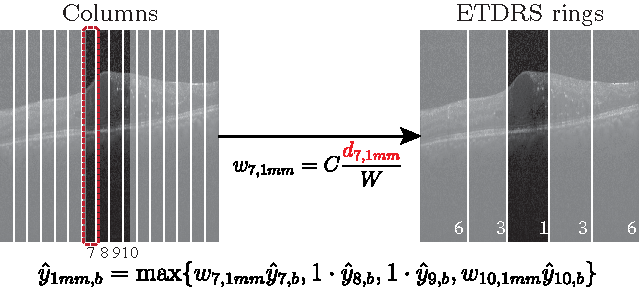
\includegraphics[width=.8\textwidth]{Figures/columns.pdf}
%\caption{Mapping column predictions to ring predictions for the central slice of an OCT~volume. The column layout (left) is shared among all slice positions. The ring layout (right) is specific to the slice location in the volume. $w_{i,j}$ is the contribution of ring $j$ in the $i$-th column and $\haty_{i,b}$ is the prediction for ring $i$ and marker $b$.
%}
%\label{fig:columns}
%\end{figure}

\textfig[t]{1}{Figures/columns.pdf}{Mapping column predictions to ring predictions for the central slice of an OCT~volume. The column layout (left) is shared among all slice positions. The ring layout (right) is specific to the slice location in the volume. $w_{i,j}$ is the contribution of ring $j$ in the $i$-th column and $\haty_{i,b}$ is the prediction for ring $i$ and marker $b$.}{fig:columns}

Specifically, instead of training our method to produce different outputs depending on the slice location, we predefined a partition of 2D OCT slices into image columns\sidenote{See \Cref{fig:columns}, left.}. That is, we will train our method to produce predictions for each of these columns, regardless of the specific slice location within the volume. At the end of this section we describe the straightforward post-processing mapping from column-level predictions to the ETDRS rings (as shown in \Cref{fig:columns} left).


\subsection{Model}

\begin{margintable}[]\small
\caption{List of variables and their description}
\label{tab:var_list_loc}
\begin{tabular}{@{}cl@{}}
\toprule
\textbf{Var.}       & \textbf{Description}                                                                                         \\ \midrule
$H$            & Slice height                                                                              \\
$W$            & Slice width                                                                           \\
$C$            & Num. of columns                                              \\
$\x$           & 2D OCT slice                                                                                        \\
$\x'$          & Flipped OCT slice                                                                                \\
$\haty$        & Probs. for $\x$                                                \\
$\haty'$       & Probs. for $\x'$                                   \\
$\haty_{0,b}$  & Prob. of~$b$ in the slice                                              \\
$\haty_{c, b}$ & Prob. of~$b$ in column~$c$                                                        \\
$\y_0$         & Slice-level annotations                                                                             \\
$\y_{0,b}$     & Annotations for $b$                                                           \\
$\z$           & Feature map                                                                      \\
$\d_0$         & OCT slice descriptor               \\
$\d_c$         & Column~$c$ descriptor    \\ \bottomrule
\end{tabular}
\end{margintable}

Formally, we partition a 2D OCT slice,~$\x$, into $C$ equally spaced columns. We wish to train a model~$f:[0,1]^{H\times W} \to [0,1]^{(1+C)\times B}$ that maps $\x$ to a collection of probabilities~$\haty$, where $B$~is the number of different possible types of markers to be found. For each marker~$b\in B$, the collection~$\haty$ contains both the probability of presence of~$b$ in the entire OCT slice,~$\haty_{0,b}$, and the probability of presence of~$b$ in each column~$c\in C$, denoted~$\haty_{c, b}$. Our training data is made of tuples~$(\x, \y_0)$, with OCT slice~$\x$ and corresponding slice-level annotations~$\y_0\in\{0, 1\}^B$ with no reference whatsoever to the ring or column in which they are located.
%\begin{figure}[t]
%\centering
%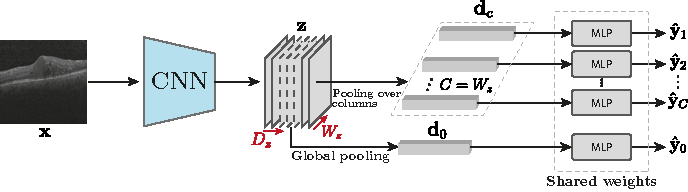
\includegraphics[width=\textwidth]{Figures/architecture.pdf}
%\caption{Our proposed network architecture: usage of partial pooling to extract information from the feature map to infer location outputs with a set of shared-weight MLPs.}
%\label{fig:architecture}
%\end{figure}

\plainwidefig[t]{1}{Figures/architecture.pdf}{Proposed network architecture: usage of partial pooling to extract information from the feature map to infer location outputs with a set of shared-weight MLPs.}{fig:architecture}

\Cref{fig:architecture} depicts our model architecture. The input OCT slice is processed by a CNN which produces a feature map~$\z \in \real^{D_z\times H_z\times W_z}$ with width equal to the number of columns~$C = W_z$. We then apply a number of pooling operations over the feature map~$\z$ to describe the entire OCT slice as well as every column~$c$. In particular, to identify markers that may appear as large or small in a given image, we set the descriptor of the entire OCT slice to be a $2D_z$-dimensional vector~$\d_0=[\avgpool(\z), \maxpool(\z)]$ obtained as the concatenation of average pooling and maximum pooling over the spatial dimensions of~$\z$. Likewise, the descriptor of every column~$c$ is another $2D_z$-dimensional vector~$\d_c=[\avgpool(\z_{\cdot,\cdot,c}), \maxpool(\z_{\cdot,\cdot,c})]$ obtained as the concatenation of the two pooling operators acting on the corresponding column of~$\z$. The descriptor vectors are then processed by a multi-layer perceptron (MLP) followed by an element-wise sigmoid activation to produce the final probabilities,
\begin{equation}
    \haty_0 = \sigma\left(\textrm{MLP}(\d_0)\right),\quad \quad 
    \haty_c = \sigma\left(\textrm{MLP}(\d_c)\right) \quad \forall c.
\end{equation}



\subsection{Training}

We use a combination of three loss terms to train our model. The first term uses the standard \autoindex{binary cross entropy} (BCE) of the slice-level predictions~$\haty_0$ with the slice-level ground-truth annotations~$\y_0$,
\begin{equation}
    \ell_1(\haty, \y_0) = \sum_{b} \textrm{BCE}(\haty_{0,b}, \y_{0,b}).
    \label{eq:l1}
\end{equation}

The second term incorporates constraints on column-level predictions based on the image-level ground-truth. Specifically, when a biological marker is not present in the input image, $\y_{0,b} = 0$, we penalize high predicted probabilities for~$b$ in all the columns. On the other hand, if the marker is present, $\y_{0,b}=1$, we encourage a high probability for~$b$ for at least one column. Formally, we compute,
\begin{equation}
    \ell_2(\haty, \y_{0,b}) = -\sum_b (1-\y_{0,b})\dfrac{1}{C}\sum_c \log (1-\haty_{c,b}) - \sum_b \y_{0,b}\max_c \log \haty_{c,b}.
    \label{eq:l2}
\end{equation}
The last term imposes invariance to horizontal symmetry on the column-level probabilities. When our model receives a horizontally flipped image~$\x'$, the predicted column-level probabilities~$\haty'$ should also be flipped, and therefore $\haty_{c,b}$~should be equal to~$\haty'_{C-c,b}$ for all~$b$. To this end, we penalize a symmetric KL~divergence\index{KL divergence} between the corresponding probabilities,
\begin{equation}
    \ell_3(\haty, \haty') = \dfrac{1}{2}\sum_{c, b} 
        \left(
            \infdiv{\haty_{c, b}}{{\haty'_{C-c, b}}} +
            \infdiv{\haty'_{c, b}}{{\haty_{C-c, b}}}
        \right).
\end{equation}

Specifically, $\ell_3$ incorporates the symmetry of the ETDRS rings we wish to induce in our model\sidenote{The addition of $\ell_3$ doubles the effective size of the training dataset and of the batches. However, this does not hurt performance as long as the new batches fit in GPU memory.}. Note that the desired horizontal symmetry cannot be obtained by random horizontal image flipping augmentation, however, as $\ell_3$ enforces predictions on the columns to be consistent regardless of whether the image is flipped or not.
Using a similar symmetry argument for $\ell_1$ and~$\ell_2$, our final loss is,
\begin{equation}
\label{eq:combinedLoss}
    \mathcal{L}(\haty, \haty', \y_0) =
        \ell_1(\haty, \y_0) + \ell_1(\haty', \y_0) + \ell_2(\haty, \y_0) + \ell_2(\haty', \y_0) + \ell_3(\haty, \haty'),
\end{equation}
where $\haty$~ and $\haty'$ are the predicted probabilities for the input image~$\x$ and corresponding horizontally-flipped version~$\x'$, respectively. \Cref{fig:loss_drawing} shows a graphical explanation for $\ell_2$ and $\ell_3$.
%\begin{figure}[t]
%\centering
%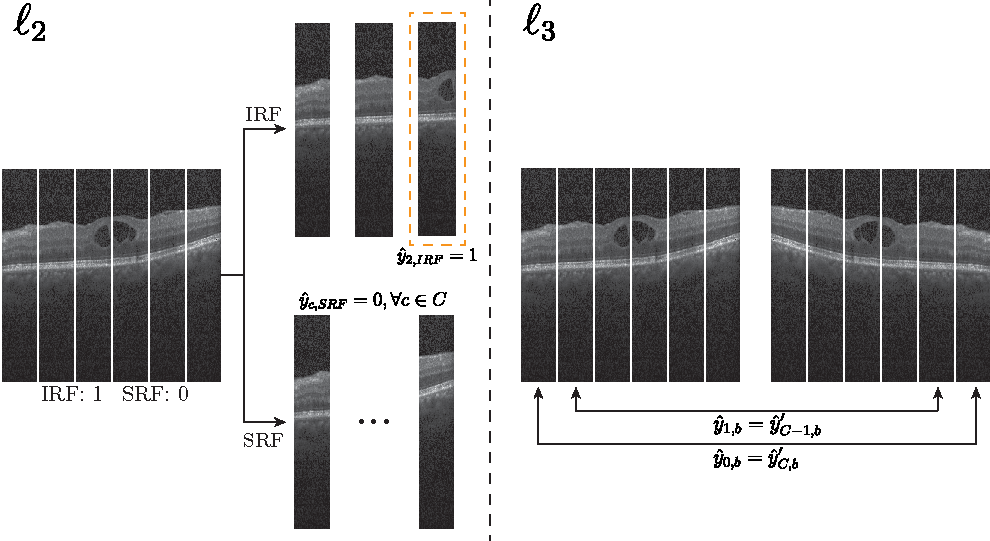
\includegraphics[width=0.85\textwidth]{Figures/loss_drawing.pdf}
%\caption{Graphical explanation for $\ell_2$ and $\ell_3$ in a slice where IRF is present and SRF is not. In this example, with $\ell_2$, we enforce that IRF must be present in at least one column while SRF is not found anywhere. With $\ell_3$ we incorporate symmetry consistency among the flipped and the non-flipped slices.}
%\label{fig:loss_drawing}
%\end{figure}

\textfig{1}{Figures/loss_drawing.pdf}{Graphical explanation for $\ell_2$ and $\ell_3$ in a slice where IRF is present and SRF is not. In this example, with $\ell_2$, we enforce that IRF must be present in at least one column while SRF is not found anywhere. With $\ell_3$ we incorporate symmetry consistency among the flipped and the non-flipped slices.}{fig:loss_drawing}


\subsection{Inference}
At test time, we can infer the layout of ETDRS rings in an OCT slice once a slice is evaluated by our network. This correspondence is not one-to-one, as a single ring usually contains several columns, and one column may be shared between two rings. To thus produce ring-level predictions, we compute the maximum of the probabilities of the columns contained in each ring. For columns spanning two rings, we weigh the contribution of the column by the proportion of the column inside each ring, as shown in \Cref{fig:columns}.
